\documentclass[a4paper,10pt]{article}
\usepackage[latin1]{inputenc}
\usepackage[english]{babel}
\usepackage{amsmath}
\usepackage{amsfonts}
\usepackage{amssymb}

\usepackage{titling}
\usepackage{nomencl}
\usepackage{siunitx}
\usepackage[style=ieee,backend=bibtex,defernumbers=true]{biblatex}
\usepackage{endnotes}

\usepackage{graphicx}
\usepackage{color}

\usepackage{booktabs}
\usepackage{threeparttable}
\usepackage{fancyhdr}

\usepackage{varioref}
\usepackage{textcomp}
\usepackage{xspace}
\usepackage[activate={true,nocompatibility},final,tracking=true,kerning=true,spacing=true,factor=1100,stretch=10,shrink=10]{microtype}
% activate={true,nocompatibility} - activate protrusion and expansion
% final - enable microtype; use "draft" to disable
% tracking=true, kerning=true, spacing=true - activate these techniques
% factor=1100 - add 10% to the protrusion amount (default is 1000)
% stretch=10, shrink=10 - reduce stretchability/shrinkability (default is 20/20)

% Reduce tracking around small caps to 40%
\SetTracking{encoding={*}, shape=sc}{40}
\newcommand{\Textregistered}{\textsuperscript{\textregistered}\xspace}
\newcommand{\Texttrademark}{\texttrademark\xspace}

\newcommand{\s}{\si{\second}\xspace}
\newcommand{\W}{\si{\watt}\xspace}
\newcommand{\V}{\si{\volt}\xspace}
\newcommand{\A}{\si{\ampere}\xspace}
\newcommand{\Ohm}{\si{\ohm}\xspace}
\renewcommand{\H}{\si{\henry}\xspace}
\newcommand{\mH}{\si{\milli\henry}\xspace}
\newcommand{\Nm}{\si{\newton\metre}\xspace}
\newcommand{\rps}{\si{\radian\per\second}\xspace}
\newcommand{\Vspr}{\si{\volt\second\per\radian}\xspace}
\newcommand{\NmpA}{\si{\newton\metre\per\ampere}\xspace}
\newcommand{\Nmspr}{\si{\newton\metre\radian\per\second}\xspace}
\newcommand{\RPM}{\text{RPM}\xspace}

\newcommand{\DC}{\textsc{dc}\xspace}
\newcommand{\EMF}{\textsc{emf}\xspace}
\newcommand{\TRBDFII}{\textsc{tr-bdf\footnotesize2}\xspace}
\newcommand{\odetwothreebt}{ode\oldstylenums{23}bt\xspace}
\newcommand{\SW}[1]{\textsc{sw\footnotesize#1}\xspace}

% Document info.
\author{Russell Maguire}
\title{E27 Lab Report}
\date{\today}

% Path to images.
\graphicspath{{img/}}

% Setup nomenclature.
\renewcommand\nomgroup[1]{
    \ifthenelse{\equal{#1}{A}}{
        \item[\textbf{Acronyms}]}{
    \ifthenelse{\equal{#1}{B}}{
        \item[\textbf{Variables}]}{
}}}
\newcommand{\nomindex}[2][]{
    \hspace*{\fill}
    \makebox[9em][l]{\ifthenelse{\equal{#1}{}}{#2}{#2~\textbf{or}~#1}}
}
\makenomenclature

% Setup bibiliography.
\DeclareBibliographyCategory{cited}
\AtEveryCitekey{\addtocategory{cited}{\thefield{entrykey}}}
\addbibresource{bibliography}
\nocite{*}

% Header and footer.
\pagestyle{fancy}
\fancyhf{}
\lhead{\thetitle}
\rhead{\theauthor}
\cfoot{\thepage}
\renewcommand{\headrulewidth}{0pt}
\renewcommand{\footrulewidth}{0pt}

\begin{document}
    
% Title page.
\begin{titlepage}
    \centering
    \vspace*{\fill}
    
\includegraphics[width=0.5\textwidth]{Durham}\\
    \vspace*{\fill}
    \LARGE\thetitle\\
    \large\theauthor\\
    \large L2 Electrical Engineering\\
    \large\thedate\\
    \vspace*{\fill}
\end{titlepage}

% Contents page.
\pagenumbering{roman}
    
\tableofcontents
    
% Acronyms
\nomenclature[A0]{\DC}{Direct current}
\nomenclature[A1]{\EMF}{Electromotive force}
\nomenclature[A2]{\textsc{rpm}}{Revolutions per minute}
\nomenclature[A3]{\SW}{Switch}

% Variables
\nomenclature[B00]{$B$}{Load torque constant \nomindex{\Nmspr}}
\nomenclature[B01]{$E$}{Motor back \EMF \nomindex{\V}}
\nomenclature[B02]{$I$}{Current \nomindex{\A}}
\nomenclature[B03]{$K$}{Motor \EMF constant \nomindex[\Vspr]{\NmpA}}
\nomenclature[B04]{$L$}{Inductance \nomindex{\H}}
\nomenclature[B05]{$N$}{Motor speed \nomindex{\RPM}}
\nomenclature[B07]{$P$}{Power \nomindex{\W}}
\nomenclature[B07]{$R$}{Resistance \nomindex{\Ohm}}
\nomenclature[B08]{$T$}{Torque \nomindex{\Nm}}
\nomenclature[B09]{$V$}{Supply voltage \nomindex{\V}}
\nomenclature[B10]{$t$}{Time \nomindex{\s}}
\nomenclature[B11]{$\omega$}{Motor speed \nomindex{\rps}}

\printnomenclature

% Main matter.
\clearpage
\pagenumbering{arabic}

\begin{abstract}
    In this report, it is described how the MathWorks\Textregistered 
    Simulink\Textregistered and SimScape\Texttrademark graphical packages were 
    used to model the way electrical and mechanical properties of a separately 
    excited \DC motor changed in time. \textcolor{red}{TODO: COMPLETE ME}
    
\end{abstract}

\section{Introduction}

\textcolor{red}{TODO}

\section{Background}

The most general form of \DC motor is a separately excited \DC motor, where the 
motor consists of two distinct parts---the stator field and armature---which 
each have their own independent \DC voltage source. Under constant field 
operation, the magnetic field produced by current flowing through the field 
windings is unchanging. As current flows through windings in the armature, an 
electric field is produced which interacts with the static magnetic field. This 
interaction exerts an electromagnetic torque $T_e$ on the armature, 
proportional to the armature current $I_a$.

\begin{equation}  \label{eq:T}
    T_e = K I_a ~\Leftrightarrow~ I_a = \frac{T_e}{K} \\
\end{equation}

The constant that relates electromagnetic torque is composed of the field 
current $I_f$ and the coupling inductance between the field and stator windings 
$L_{af}$ as follows:

\begin{equation} \label{eq:K}
    K = L_{af} I_f \\
\end{equation}

Figure~\vref{fig:Circuit} contains the circuit diagram of a separately excited 
\DC motor subjected to a load torque $T_L$. When there is a net torque on the 
armature the motor accelerates to some non-zero rotational speed. Consequently, 
the armature current moves relative to the stator field, so a back \EMF is 
induced across the armature windings such that it opposes its supply voltage in 
accordance with Faraday and Lenz's laws. The same motor constant from 
Equation~\ref{eq:K} relates the back \EMF $E$ to the rotational speed $\omega$.

\begin{equation}  \label{eq:omega}
    E = K \omega ~\Leftrightarrow~ \omega = \frac{E}{K} \\
\end{equation}

\begin{figure}[h]
    \centering
    \def\svgwidth{0.6\textwidth}
    \input{img/Circuit.pdf_tex}
    \caption{Circuit diagram of a seperately excited \DC motor.}
    \label{fig:Circuit}
\end{figure}

During the initial phase of operation, the rotational speed of the armature is 
small. As a result---according to Equation~\ref{eq:omega}---the back \EMF is 
similarly small. As armature windings do not have a large resistance, this 
results in a potentially damaging current. To compensate the starting 
resistance $R_{st}$ in  Figure~\ref{fig:Circuit} is set to some sufficiently 
large value to limit the current in the armature.

Applying Kirchoff's voltage law to the left hand side of 
Figure~\ref{fig:Circuit}, an equation linking all the electrical properties of 
the armature is found:

\begin{equation}  \label{eq:ERst}
    E = V - I_a(R_a + R_{st}) \\
\end{equation}

However, under normal operation after the motor has started, the resistance 
$R_{st}$ is taken out of the armature to achieve a greater electromagnetic 
torque. The following equation describes how the electrical properties of the 
armature are related under normal operation:

\begin{equation}  \label{eq:E}
    R_{st} = 0~\Ohm ~\Rightarrow~ E = V - I_a R_a \\
\end{equation}

\section{Methods}

The Simulink package and SimScape library produced by MathWorks were used to 
model the behaviour of a \DC motor system with a two step motor starter, using 
an implementation of \TRBDFII developed in \cite{bank1985transient}. The 
process of implementing this method was described in \cite{hosea1996analysis}. 
In Simulink, \TRBDFII is used in the \odetwothreebt solving method. The block 
diagram of the model the solver was used on is documented in 
Figure~\vref{fig:Model}. 

\begin{figure*}[b]
    \centering
    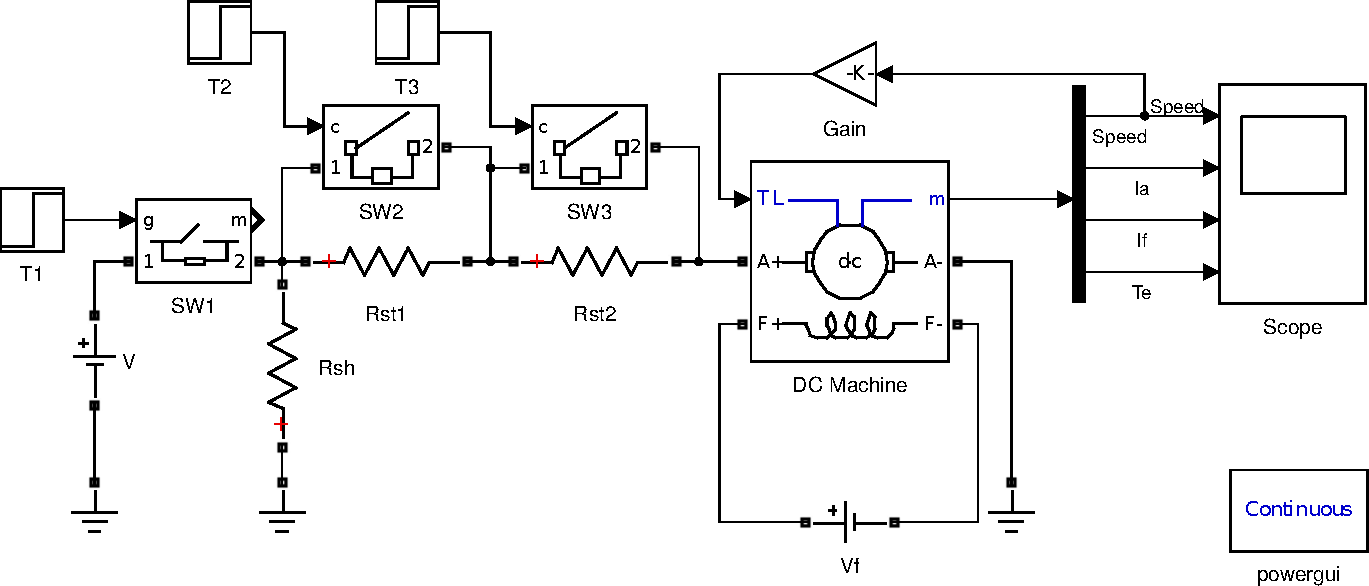
\includegraphics[width=\textwidth]{Model}
    \caption{Block diagram of the Simulink model.}
    \label{fig:Model}
\end{figure*}

The \DC machine was configured with the resistance and inductance of the 
armature and field windings given in Table~\vref{table:Parameters}. The 
electrical inputs for these windings were implemented using external \DC 
voltage 
sources; these were also given in Table~\ref{table:Parameters}. For monitoring 
purposes, the outputs of the motor were armature current, field current,
electromagnetic torque and rotational speed.

\begin{table*}[t]
    \centering
    \begin{threeparttable}
        \caption{Defining parameters of \DC motor system.}
        \label{table:Parameters}
        \begin{tabular}{llrl}
            \toprule
            \multicolumn{4}{l}{\textbf{Armature Components}} \\
            \hspace{1em}$V$   & Supply voltage      & 240 & \V \\
            \hspace{1em}$R_a$ & Armature resistance & 1.6 & \Ohm \\
            \hspace{1em}$L_a$ & Armature inductance &  12 & \mH \\
            \midrule
            \multicolumn{4}{l}{\textbf{Field Components}} \\
            \hspace{1em}$V_f$    & Field voltage     &  240 & \V \\
            \hspace{1em}$R_a$    & Field resistance  &  240 & \Ohm \\
            \hspace{1em}$L_a$    & Field inductance  &  120 & \H \\
            \hspace{1em}$L_{af}$ & Mutual inductance & 1.65 & \H \\
            \midrule
            \multicolumn{4}{l}{\textbf{Load Characteristics}} \\
            \hspace{1em}$T_{e0}$   & Initial torque         & 45       & \Nm \\
            \hspace{1em}$\omega_0$ & Initial speed          &  1       & \rps \\
            \hspace{1em}$B$        & Load constant\tnote{*} & 0.247969 & \Nmspr 
            \\
            \bottomrule
        \end{tabular}
        \begin{tablenotes}
            \item[*]See Equation~\vref{eq:B}.
        \end{tablenotes}
    \end{threeparttable}
\end{table*}

\subsection{Electric Hoist Load}

The motor in the simulation was loaded with an electric hoist--type load. The 
rotational speed $\omega$ was used to described the load torque $T_L$ 
using the following relationship:

\begin{equation} \label{eq:B}
    T_L = B\omega \\
\end{equation}

This was modelled by connecting the speed output of the \DC machine to the 
torque load input via a constant gain block, configured with multiplicative 
gain $B$ given in Table~\ref{table:Parameters}. This can be seen in the top 
right of Figure~\ref{fig:Model}.

\subsection{Motor Starter}

The motor starter in this model---represented as a variable resistor in 
Figure~\ref{fig:Circuit}---was modelled using three switches in series with the 
armature winding. Two of the switches were parallel to a resistor, such that 
all current flowed through the resistor when the switch was open: when the 
switch was closed the current experienced no resistance. 
Figure~\vref{fig:Starter} shows the circuit diagram of the network implemented, 
at the start of the simulation.

\begin{figure}[h]
    \centering
    \def\svgwidth{0.6\textwidth}
    \input{img/Starter.pdf_tex}
    \caption{Circuit diagram of the motor starter used in the model.}
    \label{fig:Starter}
\end{figure}

An ideal switch was used to model \SW{1} and circuit breakers were used to 
model \SW{2} and \SW{3}. These were closed at 0.5~\s, 2.5~\s and 3.5~\s 
respectively using step blocks; this can be seen in Figure~\vref{fig:Model}. 
The 0.5~\s delay before powering the armature winding gave the field current 
and armature mechanics sufficient to stabilise, whilst the other two switches 
removed the starting resistance in two steps.

However, because the 120~\H inductance of the field winding was too large for 
the field current to reach a stable value in 0.5~\s, the \DC machine was 
configured with a stable initial field current. Applying Ohm's law to the right 
hand side of Figure~\ref{fig:Circuit}, the following field current was found:

\begin{align*}
    I_f &= \frac{V_f}{R_f} \\
    I_f &= \frac{240~\V}{240~\Ohm} \\
    I_f &= 1~\A \\
\end{align*}

The starting resistance limited the current flowing through the armature 
winding---to prevent damage---but the current had to be sufficiently large to 
generate the initial 45~\Nm of electromagnetic torque prescribed in 
Table~\ref{table:Parameters}. Before this resistance could be calculated, the 
motor \EMF constant had to be determined. Substituting the mutual inductance 
from Table~\ref{table:Parameters} and the constant field current into 
Equation~\ref{eq:K} yielded the following result:

\begin{align*}
    K &= L_{af} I_f \\
    K &= (1.65~\H) (1~\A) \\
    K &= 1.65~\Vspr \\
\end{align*}

The maximum allowable resistance was calculated by substituting 
Equations~\ref{eq:K} and \ref{eq:omega} into Equation~\ref{eq:ERst} and 
rearranging for $R_{st}$. The initial speed of the armature was assumed to be 
1~\rps. The result after substituting the necessary values was as follows:

\begin{align*}
    K \omega &= V - \frac{T_e}{K}(R_a + R_{st}) \\
    \Leftrightarrow~ R_{st} &= \frac{V - K\omega}{T_e/K} - R_a \\
    R_{st} &= \frac{240~\V - (1.65~\Vspr)(1~\rps)}{(45~\Nm)/(1.65~\NmpA)}
        - 1.5~\Ohm \\
    R_{st} &= 7.2395~\Ohm \\
\end{align*}

\subsection{Variable Speed Operation}

Once the simulation had been run in the state defined in 
Table~\ref{table:Parameters} at a nominal speed of 1220~\RPM, the effect of 
varying speed by reducing the supply voltage was tested. The target nominal 
speed was 800~\RPM, which first had to be converted into \rps.

\begin{equation*}
    N = 800~\RPM~\Leftrightarrow~\omega = 80\pi/3~\rps
\end{equation*}

The load torque at this speed was found by substituting the speed in \rps into 
Equation~\vref{eq:B} as follows:

\begin{align*}
    T_L &= B\omega \\
    T_L &= (0.247969~\Nmspr)(80\pi/3~\rps) \\
    T_L &= \textcolor{red}{TODO}~\Nm \\
\end{align*}

From the load torque the armature could be calculated using 
Equation~\ref{eq:T}, assuming the motor was able to output enough 
electromagnetic torque to match the load torque without slipping---load torque 
and electromagnetic torque were equivalent.

\begin{align*}
    I_a &= \frac{T_e}{K} \\
    I_a &= \frac{\textcolor{red}{TODO}~\Nm}{1.65~\NmpA} \\
    I_a &= 12.590~\A \\
\end{align*}

Finally, the required supply voltage was found by substituting 
Equation~\ref{eq:omega} into Equation~\ref{eq:E} and rearranging for $V$. The 
$R_{st}$ term could be neglected, as at nominal speed the motor should have 
already started and stabilised.

\begin{align*}
    K \omega &= V - I_a R_a \\
        \Leftrightarrow~V &= K \omega + I_a R_a \\
    V &= (1.65~\Vspr)(80\pi/3~\rps) + (12.590~\A)(1.5~\Ohm) \\
    V &= 157.12~\V \\
\end{align*}

The \DC voltage source for the armature winding was reconfigured with an 
amplitude of 157.12~\V and the simulation rerun.

\section{Results and Discussion}

\textcolor{red}{TODO}

\begin{equation*}
    N = 1220~\RPM~\Leftrightarrow~\omega = 122\pi/3~\rps
\end{equation*}

\begin{align*}
    K \omega &= V - I_a R_a \\
    \Leftrightarrow~ I_a &= \frac{V - K \omega}{R_a} \\
    I_a &= \frac{240~\V - (1.65~\Vspr)(122\pi/3~\rps)}{1.5~\Ohm} \\
    I_a &= 19.466~\A \\
\end{align*}


\begin{figure}[h]
    \centering
    \def\svgwidth{\textwidth}
    \input{img/Results240V.pdf_tex}
    \caption{Motor properties during simulation.}
    \label{fig:Results240V}
\end{figure}

\begin{figure}[h]
    \centering
    \def\svgwidth{\textwidth}
    \input{img/Results157V.pdf_tex}
    \caption{Motor properties during simulation with reduced supply 157.12~\V.}
    \label{fig:Results157V}
\end{figure}

\section{Conclusion}

\textcolor{red}{TODO}

% References.
\printbibliography[category=cited]
\DeclareFieldFormat{labelnumberwidth}{#1}
\printbibliography[
    notcategory=cited,omitnumbers=true,title={Bibliography}
]



\clearpage

% Appendices.

\end{document}
